%%%%% slides template
% Giovanni Ramirez (ramirez@ecfm.usac.edu.gt)
% 20200828
% Require: images/ecfmByN.png images/usacByN.jpg
%
%
% Use this option to print notes only
% \documentclass[xcolor=dvipsnames,handout,notes=only]{beamer}%
%
% Use this option to print notes and slides
% \documentclass[xcolor=dvipsnames,handout,notes=show]{beamer}%
%
% Use this option to get a printer-friendly version
% \documentclass[xcolor=dvipsnames,handout]{beamer}%
%
% Unse this option to get slides only
\documentclass[xcolor=dvipsnames,presentation]{beamer}%
%
%%%%%


%%%%% theme and coloring
% a list of themes can be found here https://hartwork.org/beamer-theme-matrix/
% I like a simple Malmoe with some modifications and color-schemes like
% dolphin for a white background, beetle for a gray background or dove for
% plain slides
%
% theme definition
\usetheme{Malmoe}
%
% definition of the presentation mode: full slides
\mode<presentation> {
% coloring for slides other options: beetle, dove
  \usecolortheme{dolphin}
% to include a slide with the table of contents
 \AtBeginSection[] {
  \begin{frame}
    \tableofcontents[currentsection]
  \end{frame} }
}
%
% definition of the handout mode: printer-friendly
\mode<handout>{
% coloring: dove is white
  \usecolortheme{dove}
% this is to print 2 slides in 1 page, other values are allowed
  \usepackage{pgfpages}
  \renewcommand\textbullet{\ensuremath{\bullet}}
  \pgfpagesuselayout{2 on 1}[letterpaper,border shrink=5mm]
% set the fontsize of the notes
  \setbeamerfont{note page}{size=\scriptsize}
% disable the slide with the table of contents
  \AtBeginSection[]{}
}
%%%%%

%%%%% personalisation
% clear all headers
\setbeamertemplate{headline}{}
% disable navigation buttons
\setbeamertemplate{navigation symbols}{}
% configure the blocks used for equations, theorems, etc
\setbeamertemplate{blocks}[rounded][shadow=true]
% clear the footline
\setbeamertemplate{footline}{}
% set the footline
\setbeamertemplate{footline}{
  \hbox{%
% left block with the shortname, it is set in the \author command
    \begin{beamercolorbox}[wd=.40\paperwidth,ht=2.25ex,dp=1ex,center]%
      {author in head/foot}%
      \usebeamerfont{author in head/foot}\insertshortauthor
    \end{beamercolorbox}%
% center block with the short title, it is set in the \title command
    \begin{beamercolorbox}[wd=.50\paperwidth,ht=2.25ex,dp=1ex,center]%
      {title in head/foot}%
      \usebeamerfont{title in head/foot}\insertshorttitle
    \end{beamercolorbox}%
% right block with the number of slides
    \begin{beamercolorbox}[wd=.10\paperwidth,ht=2.25ex,dp=1ex,right]%
      {date in head/foot}%
      \usebeamerfont{date in head/foot}
      \insertframenumber{} / \inserttotalframenumber\hspace*{1em}
    \end{beamercolorbox}}%
  \vskip0pt%
}
%%%%%

%%%%% packages
%
% language, decimal point mark
\usepackage[spanish,es-nodecimaldot]{babel}%
%
% to use only T1 scalable fonts
\usepackage[T1]{fontenc}%
\let\Tiny=\tiny% this is a proper configuration of the tiny font size
%
% to use UTF coding, other options latin1
\usepackage[utf8]{inputenc}%
%
\usepackage{array}
% special math symbols
\usepackage{latexsym,amsfonts,amsmath}%
%
% to include graphics
\usepackage{graphicx}%
% path to images
\graphicspath{ {./img/presentacion/} }
%
% to use tiks: nice to draw diagrams
\usepackage{tikz}%
\usetikzlibrary{arrows,shapes,positioning}
%
% to use SI units and physics notation
\usepackage{physics}%
\usepackage{multirow}
\usepackage{xcolor}
\usepackage{subcaption}
%
% to use hypenation
\usepackage{ragged2e}%
\let\raggedright=\RaggedRight%
%
\usepackage{dsfont}

\newcommand{\subind}[2]{{}_{#1}^{#2}}
%%%%% Talk data
%
%title
\title[Canales cuánticos PCE]% this is the short title
{Mapeos proyectivos en sistemas de varios qubits}% this is the long title
\subtitle{\bf Operaciones PCE \newline\vspace{1.4cm}}
%
% author
\author[José Alfredo de León]% this is the short name
{José Alfredo de León}% this is the long name
%
% affiliation
\institute{Asesorado por:\\Dr. Carlos Francisco Pineda Zorrilla (IFUNAM)
\newline y M.Sc. Juan Diego Chang (ECFM-USAC)}%
%
% date and information about the conference
\date{XX octubre 2021}
%%%%%


%%%%%
\makeatletter
\newenvironment{myitemize}{%
   \setlength{\topsep}{0pt}
   \setlength{\partopsep}{0pt}
   \renewcommand*{\@listi}{\leftmargin\leftmargini \parsep\z@ \topsep\z@ \itemsep\z@}
   \let\@listI\@listi
   \itemize
}{\enditemize}
\makeatother 


\begin{document}
% % % % % % % % % % % % % % % % % % % % % % % % % % % % % % % % % % % % % %
% Title and Outline
% % % % % % % % % % % % % % % % % % % % % % % % % % % % % % % % % % % % % %
\begin{frame}[plain]
  \titlepage 
  \begin{tikzpicture}[x=1mm,y=1mm,overlay,remember picture]
    \pgftransformshift{\pgfpointanchor{current page}{center}}
    \node[inner sep=0pt] (usac) at (-40,-14.5) %
    {
\includegraphics[height=14mm]{logos/ecfmByN}};
    \node[inner sep=0pt] (usac) at (39,-14.5) %
    {
\includegraphics[height=14mm]{logos/ifunam}};
    \node[inner sep=0pt] (usac) at (0,11) %
    {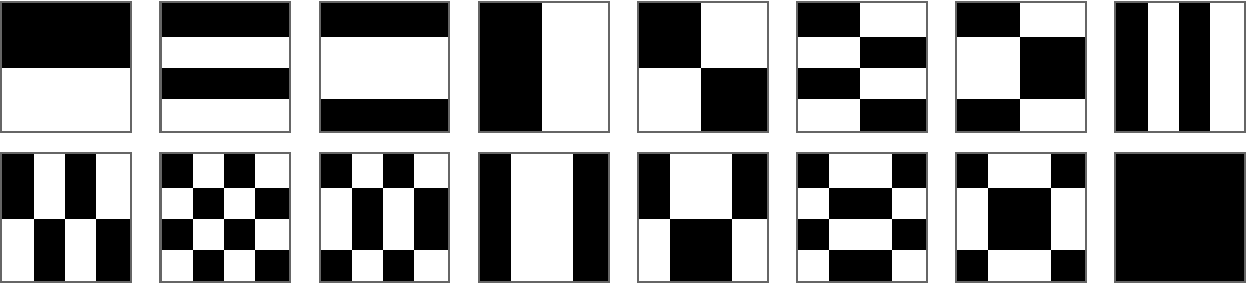
\includegraphics[height=14mm]{portada}};
  \end{tikzpicture}
\end{frame}

\begin{frame}{Agradecimientos}
	\begin{itemize}
		\item A mis padres.
		\item A mis asesores: Carlos y Juan Diego. 
		\item A Alejandro Fonseca y David Dávalos.
		\item A mis prefesores de la ECFM.
		\item A Cindy.
		\item A mis amigos Benja, Gómez, Papaya y José Guillermo.
		\item A mis amigos de la U.
	\end{itemize}
\end{frame}

\begin{frame}{Esquema de la presentación}
  \tableofcontents 
\end{frame}


% % % % % % % % % % % % % % % % % % % % % % % % % % % % % % % % % % % % % %
% Introduction and Motivation
% % % % % % % % % % % % % % % % % % % % % % % % % % % % % % % % % % % % % %
\section{Introducción}
\label{sec:Intro}
\begin{frame}[t]{Motivación}
	Con frecuencia, una descripción más precisa de un sistema
	cuántico requiere incluir la interacción con su entorno, i.e. 
	considerar al sistema como abierto.
	\begin{columns}
	\column{.5\textwidth}
		\begin{figure}
		\includegraphics<1>[width=\textwidth]{H_alone}
		\includegraphics<2>[width=\textwidth]{H_w_photons}
		\end{figure}
	\column{.5\textwidth}
		\begin{figure}
		\includegraphics<1>[width=\textwidth]{lattice}
		\includegraphics<2>[width=\textwidth]{lattice_sub}
		\end{figure}
	\end{columns}
	
	\onslide<2>{\vfill\alert{En general,
	$\ket{\psi}\ne\ket{\text{sistema}}\otimes\ket{\text{entorno}}$}}
	
\end{frame}

\begin{frame}[t]{Motivación}
	Sin embargo, los sistemas abiertos están sujetos a fenómenos de decoherencia.
	\begin{figure}
	\centering
	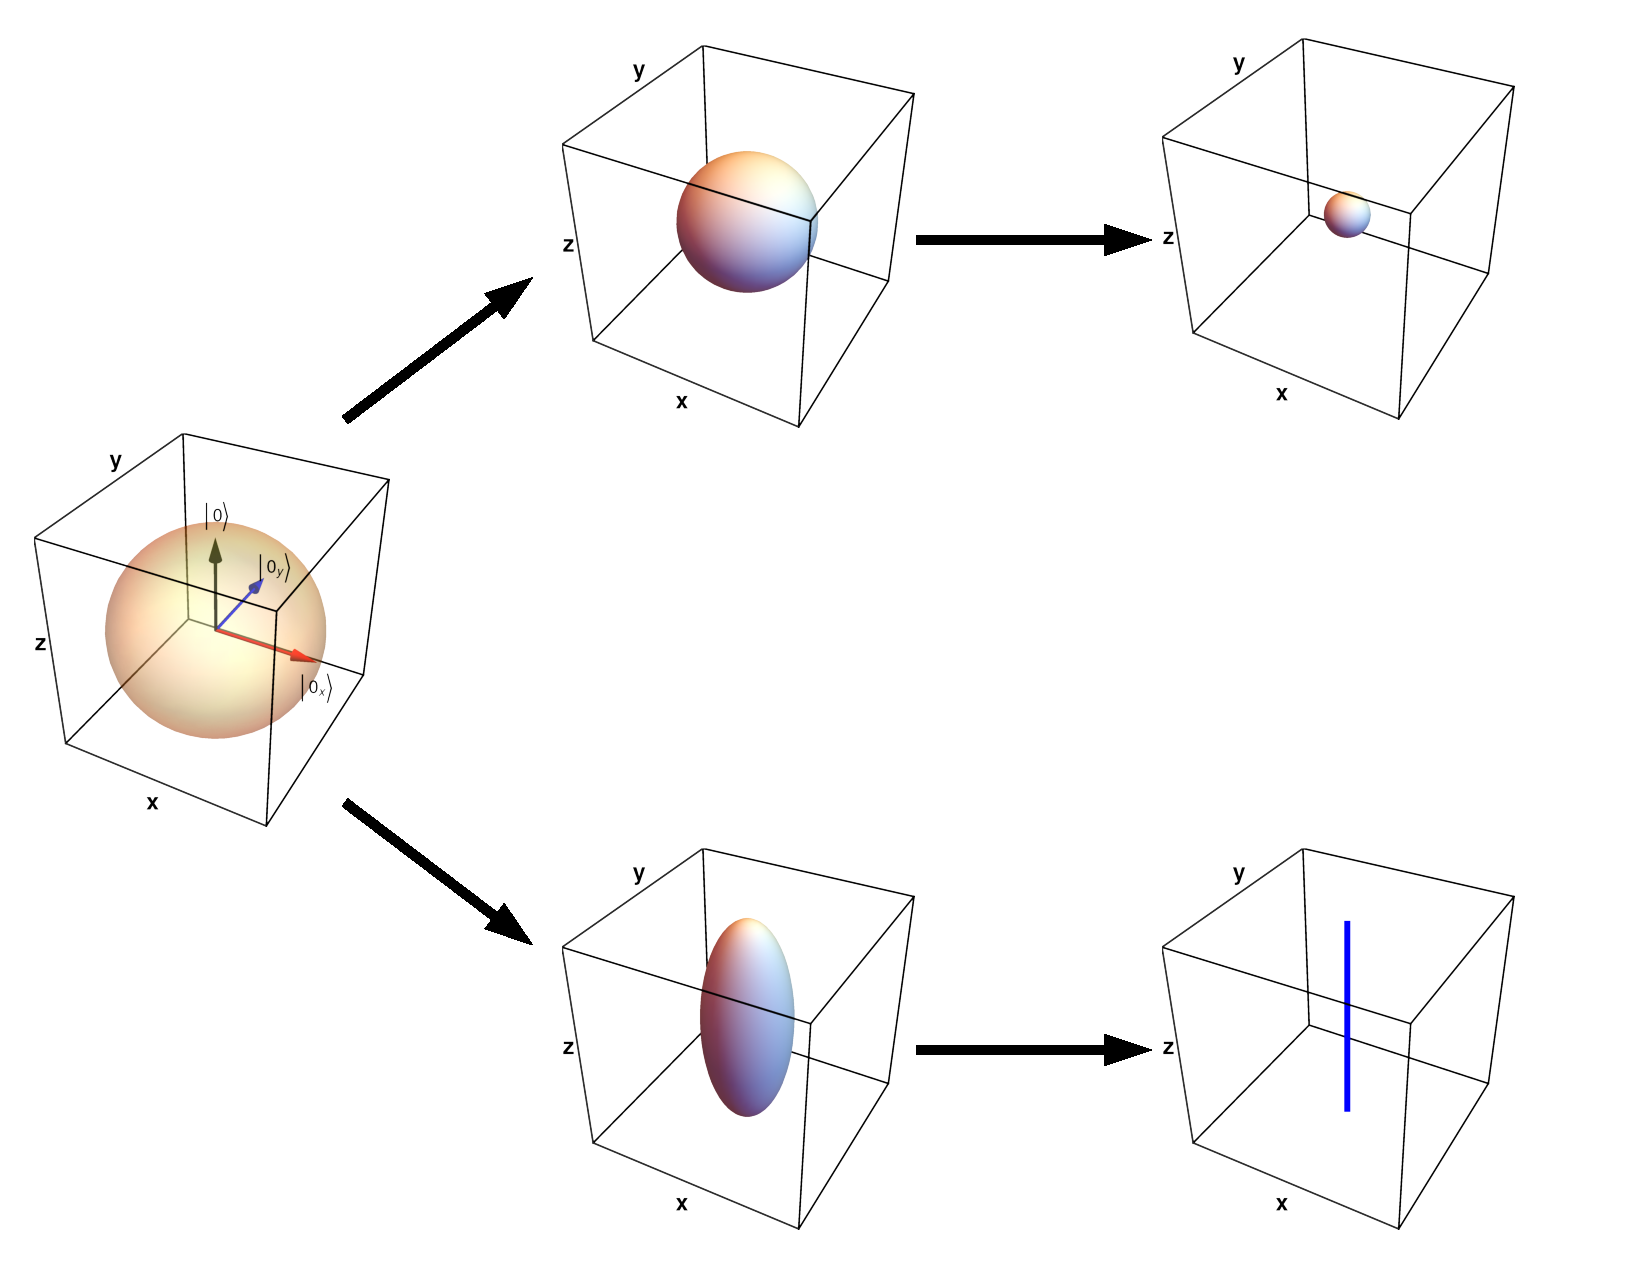
\includegraphics[width=9cm]{decoherencia_motivacion}	
	\end{figure}
\end{frame}


\section{Fundamentos teóricos}
\begin{frame}{Matriz  densidad}
Una matriz $\rho$ es una matriz densidad si y sólo si
	\begin{enumerate}
		\item $\Tr (\rho)=1$,
		\item $\matrixel{\psi}{\rho}{\psi}\geq 0$.
	\end{enumerate}	\vfill

	Por ejemplo, si un sistema se encuentra en un estado $\ket{\psi}$,
  \begin{align*}
  \rho=\dyad{\psi}{\psi}.
  \end{align*}
\end{frame}

\begin{frame}{Qubits}
Un sistema cuántico de dos niveles recibe el nombre de qubit. \vfill

	\begin{columns}	\hspace{.4cm}
	\begin{column}{0.6\textwidth}
	\begin{itemize}
		\item 1 qubit:
		\begin{align*}
			\rho &= \frac{\mathds{1}+r_1\sigma_x+r_2\sigma_y+r_3\sigma_z}{2}.
		\end{align*}	
		\item $n$ qubits:
		\begin{align*}
		\rho = \frac{1}{2^n}\sum _{j_1,\ldots,j_n=0}^3 r_{j_1,\ldots,j_n}
		\sigma_{j_1}\otimes \ldots
		\otimes\sigma_{j_n},%\qquad r_{0,\ldots,0}=1,
		\end{align*}
		$r_{j_1,\ldots,j_n}$ componentes de Pauli.
%		\item $\qty(r_1,r_2,r_3)$ especifican las coordenadas cartesianas de un 
% 		punto en la esfera de Bloch, $\alert{\rho = \qty(1,r_1,r_2,r_3)}$
	\end{itemize} \vfill
	\end{column}%\hspace{-1cm}
	\begin{column}{0.4\textwidth}  
  		\begin{center}
    		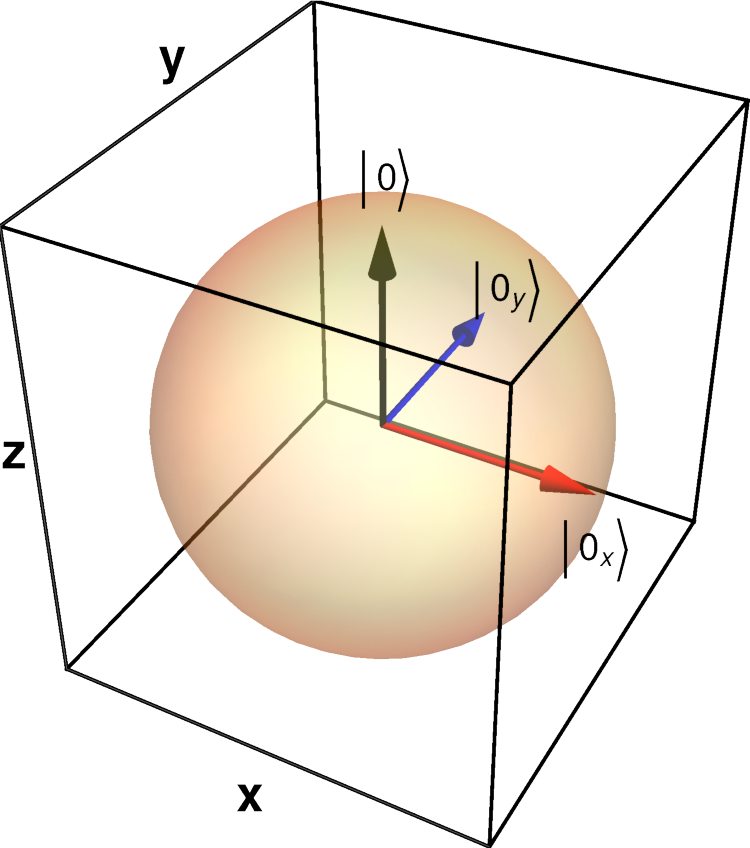
\includegraphics[width=.85\textwidth]{bloch_sphere}      
     \end{center}
		\end{column}
	\end{columns}
%	\begin{itemize}
%		\item Para $n$ qubits
%		\begin{align*}
%		\rho = \frac{1}{2^n}\sum _{j_1,\ldots,j_n=0}^3 r_{j_1,\ldots,j_n}
%		\sigma_{j_1}\otimes \ldots
%		\otimes\sigma_{j_n},\qquad r_{0,\ldots,0}=1,
%		\end{align*}
%		$r_{j_1,\ldots,j_n}$ componentes de Pauli.
%	\end{itemize}
\end{frame}

\begin{frame}{Canales cuánticos}%
  %{¿cómo describir la dinámica de los sistemas abiertos?}
  \vfill
  \begin{itemize}
  	\item La teoría de los canales cuánticos es un formalismo para describir 
  la evolución de los sistemas abiertos,
  \begin{align*}
	\mathcal{E}(\rho)=\rho'.
	\end{align*} \vfill
  \only<1>{\item Una operación lineal $\mathcal{E}$ es un canal cuántico 
  si y sólo si
	\begin{enumerate}
	\item Preserva las características de la matriz densidad
	\item Es una operación completamente positiva,
	$$
	\qty(\mathcal{E}\otimes \mathds{1})\qty[\dyad{\text{Bell}}{\text{Bell}}]\geq 0.
	$$
	\end{enumerate} \vfill
	} 
  \end{itemize}

\end{frame}	


\begin{frame}{Canales cuánticos de 1 qubit}
	Rotaciones de la esfera de Bloch
	\begin{center}
	\begin{tabular}{m{2.5cm} m{1.8cm} m{2.5cm}}
		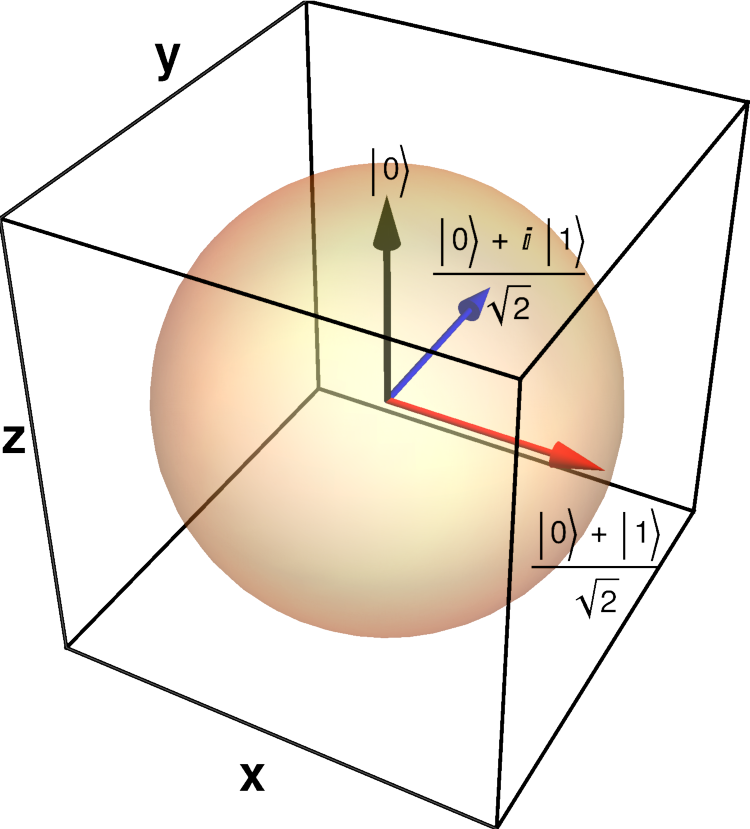
\includegraphics[width=2.5cm]{bloch_sphere2}
		& \hspace{\fill} \Large$\overset{\normalsize{R_x(\pi/3)}}{\longmapsto}$ \hspace{\fill}
		& 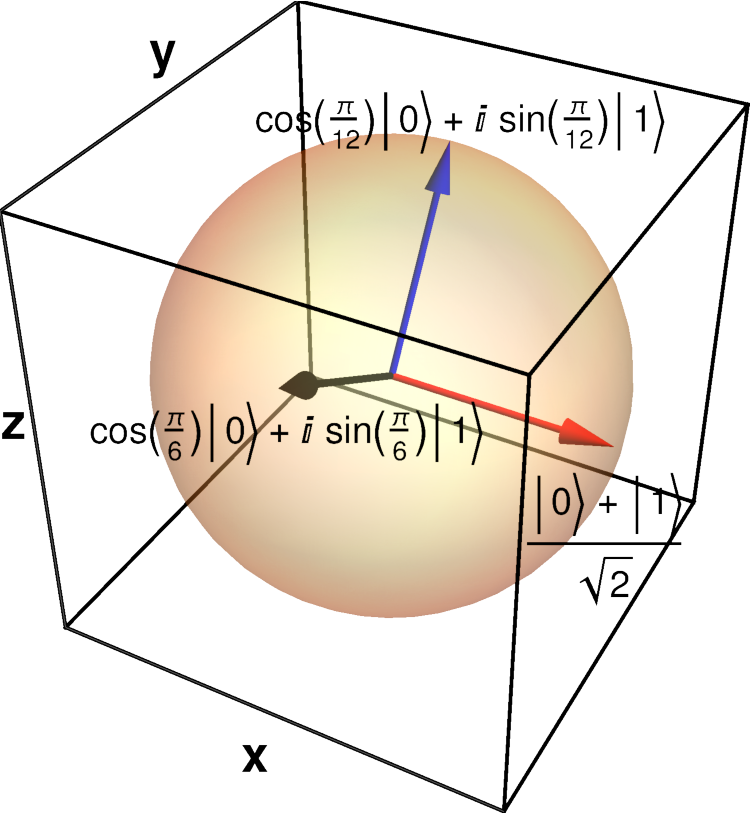
\includegraphics[width=2.5cm]{bloch_sphere_Rx_pi_medios2}
	\end{tabular}
	\end{center}
	
	Canal \textit{bit-flip}	 $\mathcal{E}$
	\begin{center}
	\begin{tabular}{m{2.5cm} m{1.8cm} m{2.5cm}}
		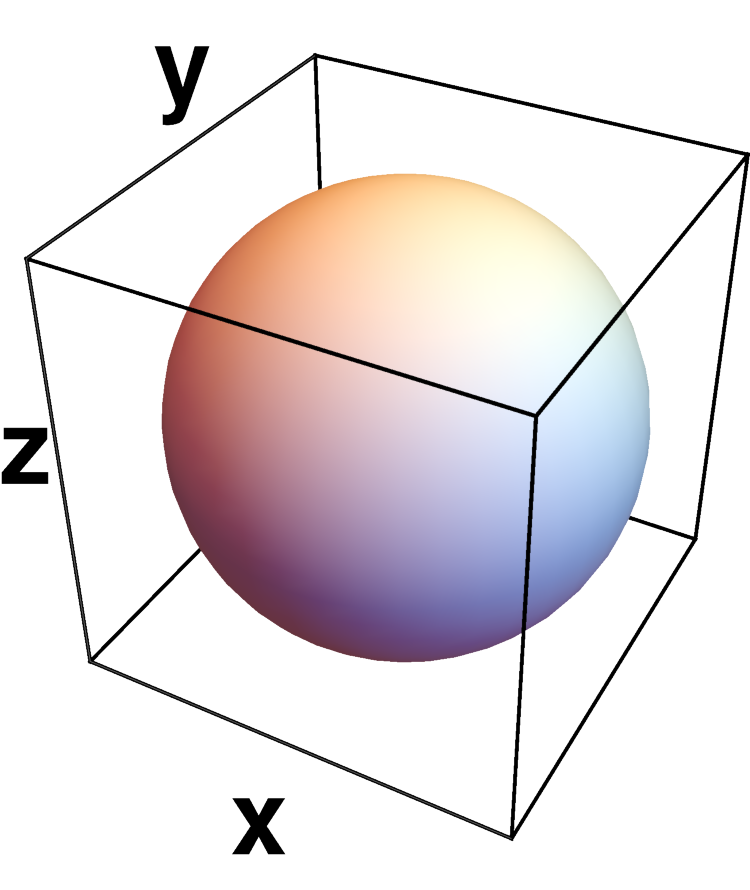
\includegraphics[width=2.5cm]{unit_sph}
		& \hspace{\fill} \Large{$\overset{\mathcal{E}}{\longmapsto}$} \hspace{\fill}
		& 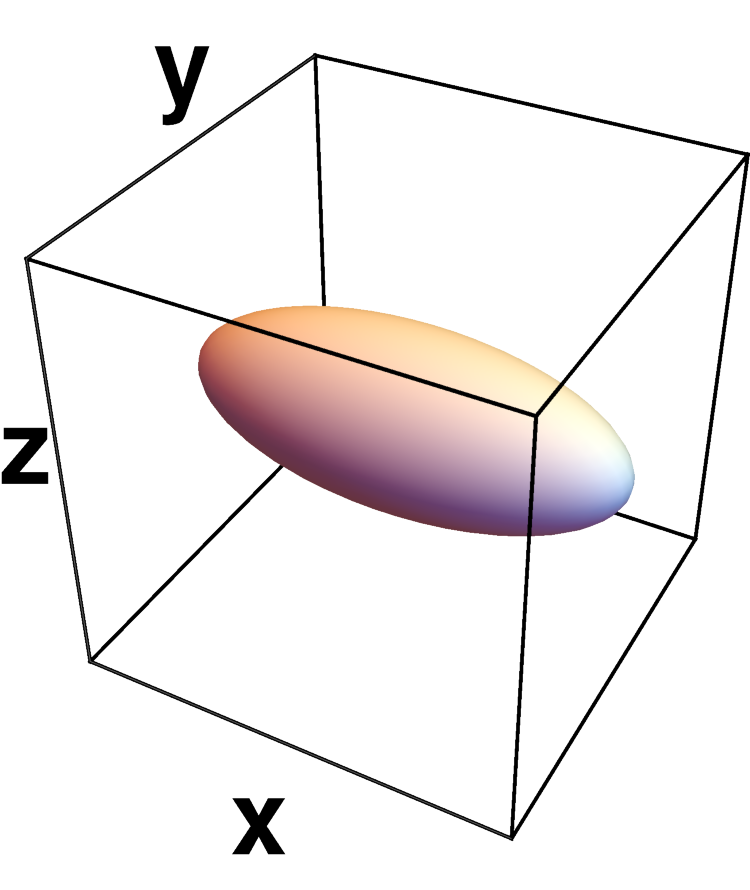
\includegraphics[width=2.5cm]{bit_flip_p0_3}
	\end{tabular}
	\end{center}
\end{frame}


% % % % % % % % % % % % % % % % % % % % % % % % % % % % % % % % % % % % % %
% Qubits
% % % % % % % % % % % % % % % % % % % % % % % % % % % % % % % % % % % % % %

\section{Operaciones PCE}

\begin{frame}{Operaciones PCE}
	\begin{itemize}
		\item<1-> Una operación PCE (\textit{Pauli component erasing}) 
		es una operación lineal que transforma a las 	componentes 
		de Pauli de la matriz densidad $\rho$ de $n$ qubits como
		\begin{align*}
		r_{j_1,\ldots,j_n}\longmapsto \tau_{j_1,\ldots,j_n}r_{j_1,\ldots,j_n},
		\qquad \tau_{j_1,\ldots,j_n}=0,1.
		\end{align*} 
	
		\item<2-> \vfill Figuras PCE: una representación geométrica
		 
		\vspace*{2mm}
		\resizebox{.75\textwidth}{!}{%
		\begin{minipage}{\textwidth}
		\begin{figure} % {{{
		\begin{center}
		\begin{tikzpicture}[x=0.5cm, y=0.5cm] % {{{
		\pgfmathsetmacro{\unitstep}{3.5}
		% Coordenadas   {{{
		\node at (-0.6,0.5) {(a)} ;
		\draw (0,0) rectangle (1,1); \node at (0.5,0.5) {$\tau_0$} ;
		\begin{scope}[shift={(0,-1)}]
		\draw (0,0) rectangle (1,1); \node at (0.5,0.5) {$\tau_1$} ;
		\end{scope}
		\begin{scope}[shift={(0,-2)}]
		\draw (0,0) rectangle (1,1); \node at (0.5,0.5) {$\tau_2$} ;
		\end{scope}
		\begin{scope}[shift={(0,-3)}]
		\draw (0,0) rectangle (1,1); \node at (0.5,0.5) {$\tau_3$} ;
		\end{scope} % }}}
%		\begin{scope}[shift={(1*\unitstep,0)}] % Identity {{{
%		% \begin{scope}[shift={(\unitstep*2,0)}]
%		\node at (-0.6,0.5) {(b)} ;
%		\fill[black] (0,0) rectangle (1,1);
%		\draw (0,0) rectangle (1,1);
%		\begin{scope}[shift={(0,-1)}] \fill[black] (0,0) rectangle (1,1); \end{scope}
%		\begin{scope}[shift={(0,-1)}] \draw (0,0) rectangle (1,1); \end{scope}
%		\begin{scope}[shift={(0,-2)}] \fill[black] (0,0) rectangle (1,1); \end{scope}
%		\begin{scope}[shift={(0,-2)}] \draw (0,0) rectangle (1,1); \end{scope}
%		\begin{scope}[shift={(0,-3)}] \fill[black] (0,0) rectangle (1,1); \end{scope}
%		\begin{scope}[shift={(0,-3)}] \draw (0,0) rectangle (1,1); \end{scope}
%		\end{scope} % }}}
		\begin{scope}[shift={(1*\unitstep,0)}] % Dephasing {{{
		\node at (-0.6,0.5) {(b)} ;
		\fill[black] (0,0) rectangle (1,1);
		\draw (0,0) rectangle (1,1);
		% \begin{scope}[shift={(0,-1)}] \fill[black] (0,0) rectangle (1,1); \end{scope}
		\begin{scope}[shift={(0,-1)}] \draw (0,0) rectangle (1,1); \end{scope}
		% \begin{scope}[shift={(0,-2)}] \fill[black] (0,0) rectangle (1,1); \end{scope}
		\begin{scope}[shift={(0,-2)}] \draw (0,0) rectangle (1,1); \end{scope}
		\begin{scope}[shift={(0,-3)}] \fill[black] (0,0) rectangle (1,1); \end{scope}
		\begin{scope}[shift={(0,-3)}] \draw (0,0) rectangle (1,1); \end{scope}
		\end{scope} % }}}
%		\begin{scope}[shift={(3*\unitstep,0)}] % Depolarization {{{
%		\node at (-0.6,0.5) {(d)} ;
%		\fill[black] (0,0) rectangle (1,1);
%		\draw (0,0) rectangle (1,1);
%		% \begin{scope}[shift={(0,-1)}] \fill[black] (0,0) rectangle (1,1); \end{scope}
%		\begin{scope}[shift={(0,-1)}] \draw (0,0) rectangle (1,1); \end{scope}
%		% \begin{scope}[shift={(0,-2)}] \fill[black] (0,0) rectangle (1,1); \end{scope}
%		\begin{scope}[shift={(0,-2)}] \draw (0,0) rectangle (1,1); \end{scope}
%		% \begin{scope}[shift={(0,-3)}] \fill[black] (0,0) rectangle (1,1); \end{scope}
%		\begin{scope}[shift={(0,-3)}] \draw (0,0) rectangle (1,1); \end{scope}
%		\end{scope} % }}}
		\begin{scope}[shift={(2*\unitstep,0)}] % (e) canal malo {{{
		\node at (-0.6,0.5) {(c)} ;
		\fill[black] (0,0) rectangle (1,1);
		\draw (0,0) rectangle (1,1);
		% \begin{scope}[shift={(0,-1)}] \fill[black] (0,0) rectangle (1,1); \end{scope}
		\begin{scope}[shift={(0,-1)}] \draw (0,0) rectangle (1,1); \end{scope}
		\begin{scope}[shift={(0,-2)}] \fill[black] (0,0) rectangle (1,1); \end{scope}
		\begin{scope}[shift={(0,-2)}] \draw (0,0) rectangle (1,1); \end{scope}
		\begin{scope}[shift={(0,-3)}] \fill[black] (0,0) rectangle (1,1); \end{scope}
		\begin{scope}[shift={(0,-3)}] \draw (0,0) rectangle (1,1); \end{scope}
		\end{scope} % }}}
		\end{tikzpicture} % }}}
%		
%		\vspace*{2mm}
		\begin{tikzpicture}[x=0.5cm, y=0.5cm] % {{{
		\pgfmathsetmacro{\unitstep}{5.8}
		\begin{scope}[shift={(0*\unitstep,0)}] % Coordenadas {{{
		\node at (-0.6,0.5) {(f)} ;
		    \foreach \x in {0,1,2,3} {
		      \foreach \y in {0,1,2,3} {
		        \begin{scope}[shift={(\x,-\y)}] 
		          \draw (0,0) rectangle (1,1); 
		          \node at (0.5,0.5) {\scalebox{.6}{$\tau_{\y,\x}$}};
		         \end{scope}
		%         \node at (0,-\y) (input\y) {$i_\y$};
		%         \node[block] at (2,-\y) (block\y) {$f_\y$};
		%         \draw[->] (input\y) -- (block\y);
		%         \draw[->] (block\y.east) -- +(0.5,0);
		    }
		    }
		\end{scope} % }}}
		\begin{scope}[shift={(1*\unitstep,0)}] % Good channel {{{
		\node at (-0.6,0.5) {(g)} ;
		    \foreach \x in {0,1,2,3} {
		      \foreach \y in {0,1,2,3} {
		        \begin{scope}[shift={(\x,-\y)}] 
		          \draw (0,0) rectangle (1,1); 
		%           \node at (0.5,0.5) {$\tau_{\y,\x}$};
		         \end{scope}
		%         \node at (0,-\y) (input\y) {$i_\y$};
		%         \node[block] at (2,-\y) (block\y) {$f_\y$};
		%         \draw[->] (input\y) -- (block\y);
		%         \draw[->] (block\y.east) -- +(0.5,0);
		    }
		    }
		\begin{scope}[shift={(0,-3)}] \fill[black] (0,0) rectangle (1,1); \end{scope}
		\begin{scope}[shift={(3,-3)}] \fill[black] (0,0) rectangle (1,1); \end{scope}
		\begin{scope}[shift={(0,0)}] \fill[black] (0,0) rectangle (1,1); \end{scope}
		\begin{scope}[shift={(3,0)}] \fill[black] (0,0) rectangle (1,1); \end{scope}
		\end{scope} % }}}
%		\begin{scope}[shift={(2*\unitstep,0)}] % Good channel {{{
%		\node at (-0.6,0.5) {(h)} ;
%		    \foreach \x in {0,1,2,3} {
%		      \foreach \y in {0,1,2,3} {
%		        \begin{scope}[shift={(\x,-\y)}] 
%		          \draw (0,0) rectangle (1,1); 
%		%           \node at (0.5,0.5) {$\tau_{\y,\x}$};
%		         \end{scope}
%		%         \node at (0,-\y) (input\y) {$i_\y$};
%		%         \node[block] at (2,-\y) (block\y) {$f_\y$};
%		%         \draw[->] (input\y) -- (block\y);
%		%         \draw[->] (block\y.east) -- +(0.5,0);
%		    }
%		    }
%		\begin{scope}[shift={(0,0)}] \fill[black] (0,0) rectangle (1,1); \end{scope}
%		\begin{scope}[shift={(0,-1)}] \fill[black] (0,0) rectangle (1,1); \end{scope}
%		\begin{scope}[shift={(2,0)}] \fill[black] (0,0) rectangle (1,1); \end{scope}
%		\begin{scope}[shift={(2,-2)}] \fill[black] (0,0) rectangle (1,1); \end{scope}
%		\begin{scope}[shift={(2,-3)}] \fill[black] (0,0) rectangle (1,1); \end{scope}
%		\end{scope} % }}}
		\end{tikzpicture} % }}}
		\end{center}
		\end{figure} % }}}
		\end{minipage}}

		\item<3-> \vfill ¿Existe una manera de caracterizar a las operaciones PCE 
		que son completamente positivas (es decir, canales cuánticos)?
	\end{itemize}
\end{frame}


\begin{frame}[t]{Método numérico}
	\only<1>{
	\begin{columns}
		\begin{column}{0.5\textwidth}
			\begin{figure}
		\centering
		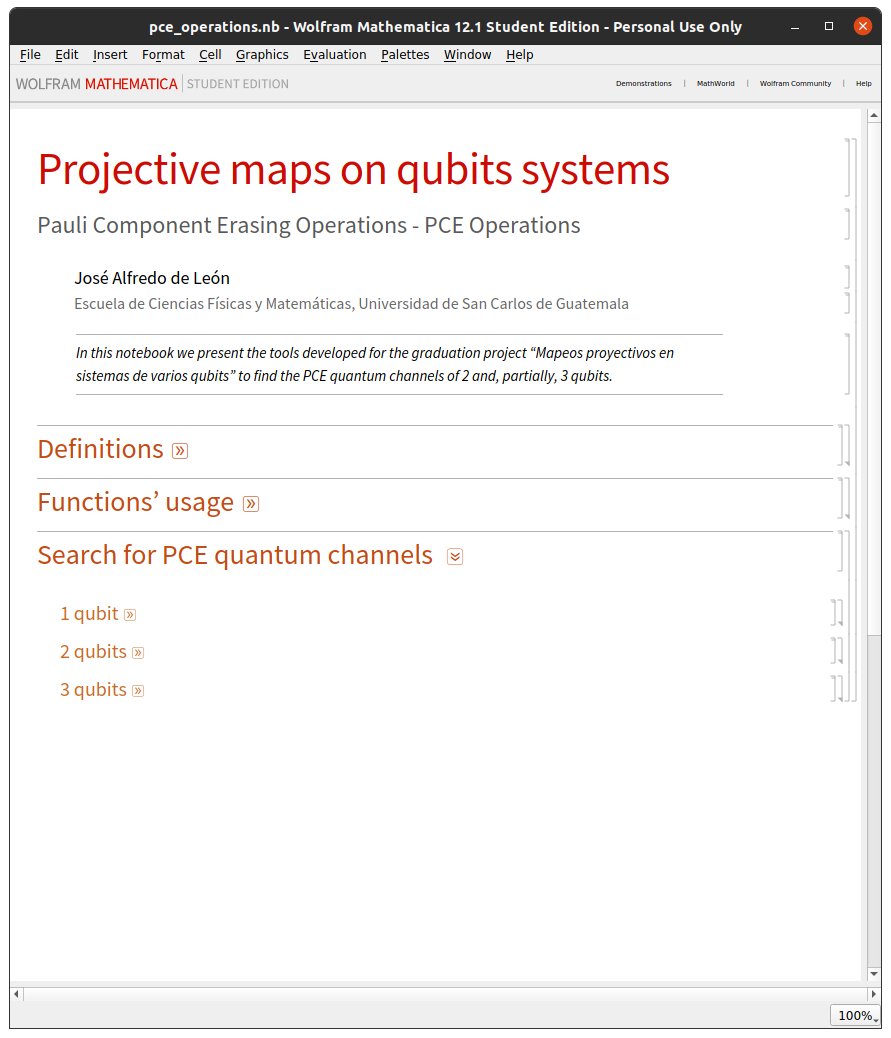
\includegraphics[width=1\textwidth]{numerico_01}
	\end{figure}		
		\end{column}
		\begin{column}{0.5\textwidth}
			\begin{figure}
		\centering
		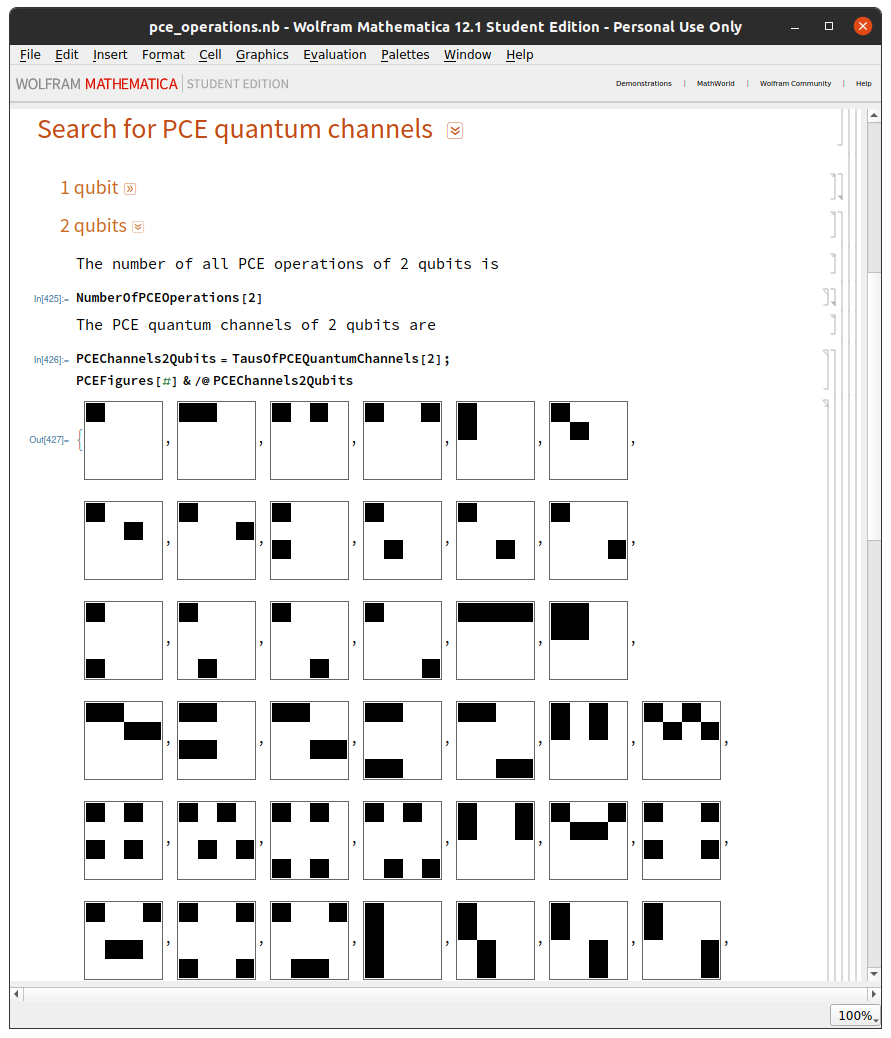
\includegraphics[width=1\textwidth]{numerico_02}
	\end{figure}		
		\end{column}
	\end{columns}		
	}
	\only<2>{
	https://github.com/deleonja/projective\_maps
	\begin{figure}
		\centering
		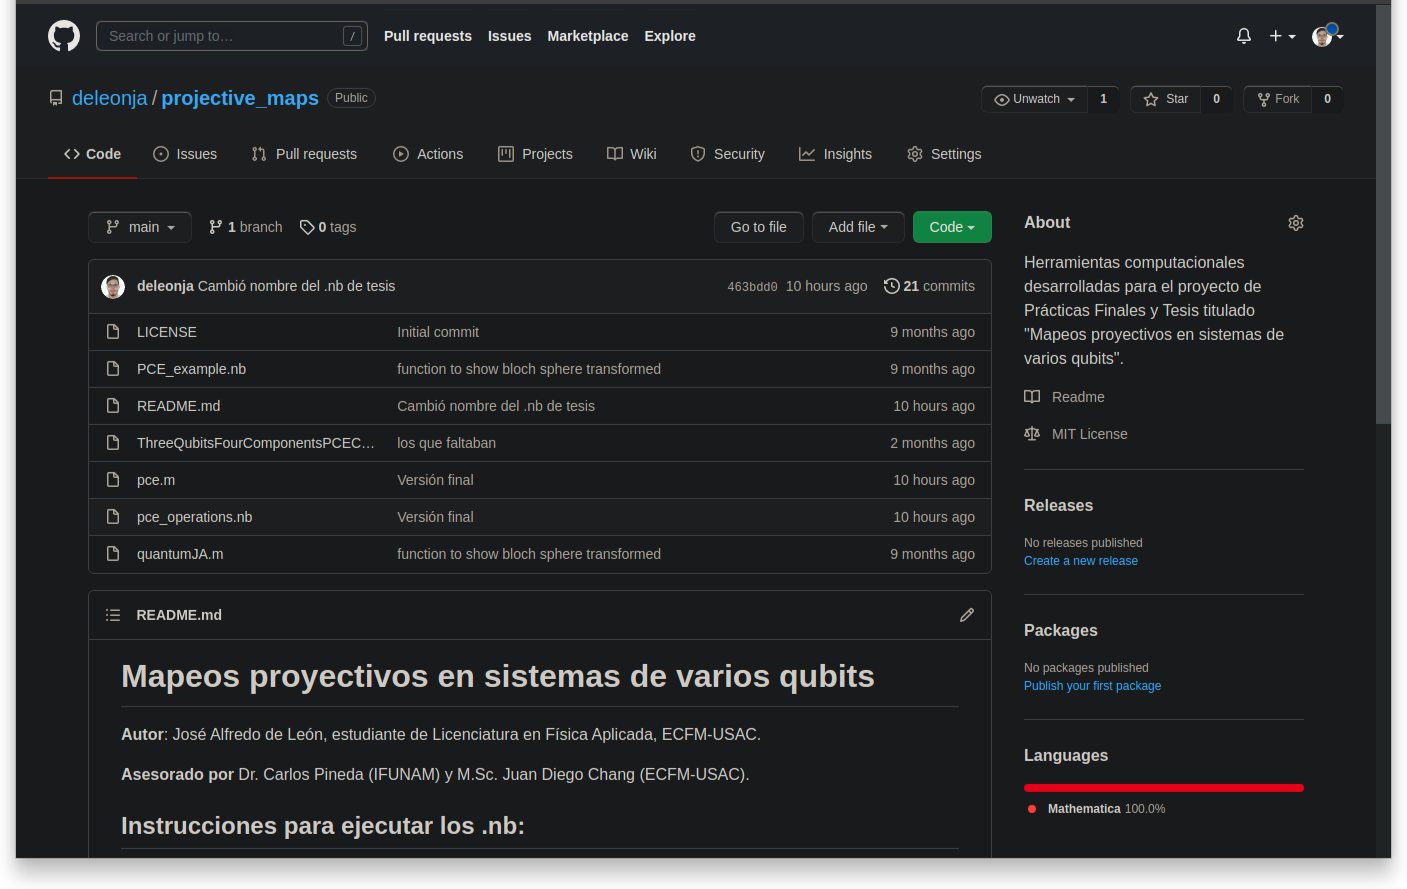
\includegraphics[width=.9\textwidth]{numerico_03}
	\end{figure}
	}
	
\end{frame}

\begin{frame}{Resultados}{Clases de equivalencia}
	Los canales cuánticos PCE pueden ordenarse en subconjuntos cuyos elementos
	son equivalente vía \vfill
	\begin{enumerate}
		\item Intercambios de partículas
		\begin{center}
		\begin{tabular}{m{1.5cm} m{1.2cm} m{1.5cm}}
		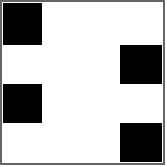
\includegraphics[height=1.5cm]{2qubits_PCE_QC_001}
		& \hspace{\fill} \Large$\longmapsto$ \hspace{\fill}
		& 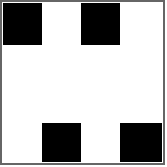
\includegraphics[height=1.5cm]{2qubits_PCE_QC_003}
		\end{tabular}
		\end{center}\vfill 
		
		\item Permutación de elementos de una base local
		
		\begin{center}
		\begin{tabular}{m{1.5cm} m{1.2cm} m{1.5cm}}
		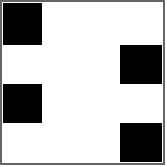
\includegraphics[height=1.5cm]{2qubits_PCE_QC_001}
		& \hspace{\fill} \Large$\longmapsto$ \hspace{\fill}
		& 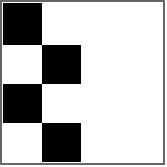
\includegraphics[height=1.5cm]{2qubits_PCE_QC_004}
		\end{tabular}
		\end{center}
	\end{enumerate}\vfill
\end{frame}

\begin{frame}{Resultados}{Regla $2^k$}
	Los canales cuánticos PCE preservan una cantidad 
	de componentes de Pauli que son potencias de dos.
	\begin{columns}[t]
		\begin{column}{0.5\textwidth}
			\begin{itemize}
				\item 1 qubit
			\end{itemize}
			\only<1>{
			Canales cuánticos PCE:
			\begin{figure}
				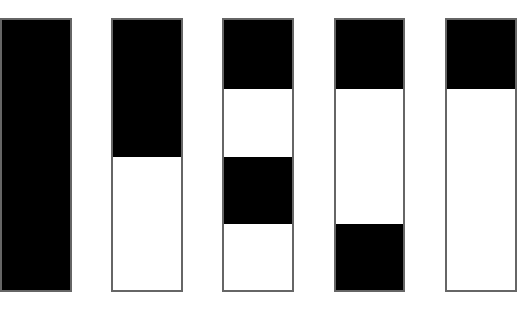
\includegraphics[height=1.4cm]{1qubit}
			\end{figure}
			Operaciones PCE no CP:
			\begin{figure}
				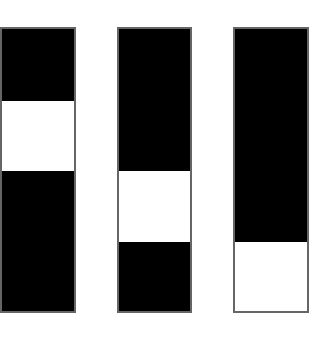
\includegraphics[height=1.6cm]{not_QC_1qubit}
			\end{figure}
			}
		\end{column} 
		\begin{column}{0.5\textwidth}		
		\begin{itemize}
		\item 2 qubits:
		\end{itemize}
		\only<1>{
		Canal cuántico PCE:
		\begin{figure}
			\centering
			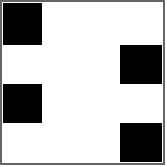
\includegraphics[height=1.5cm]{2qubits_PCE_QC_001}
		\end{figure}
		
		Operación PCE que no es CP:
		\begin{figure}
			\centering
			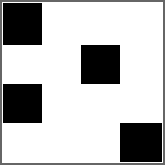
\includegraphics[height=1.5cm]{2qubits_PCE_QC_002}
		\end{figure}
		}
		\end{column}
	\end{columns}
\end{frame}

\begin{frame}{Resultados}{Regla espejo}
El número de canales cuánticos PCE en función del exponente $k$ del 
número $2^k$ de componentes de Pauli invariantes es simétrico respecto a 
$k=2n$.

	\begin{figure} % {{{
	\centering
	\begin{subfigure}[b]{0.48\textwidth}
		\centering
		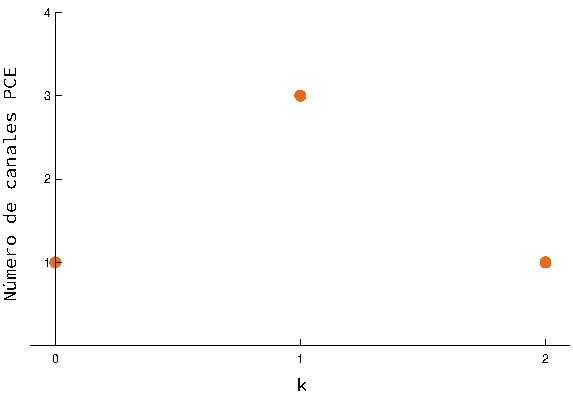
\includegraphics[width=3.7cm]	{mirroring_1qubits}
		\caption{1 qubit}
		\label{fig:mirroring_1qubit}
	\end{subfigure}
	\hfill
	\begin{subfigure}[b]{0.48\textwidth}
		\centering
		\hfill 
		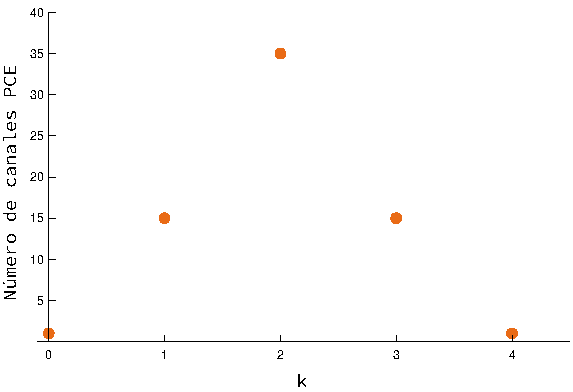
\includegraphics[width=3.7cm]{mirroring_2qubits} 
		\hfill \hfill
		\caption{2 qubits}
		\label{fig:mirroring_2qubits}
	\end{subfigure}
	\newline
	\begin{subfigure}[c]{\textwidth}
		\centering
		\hspace*{\fill}
		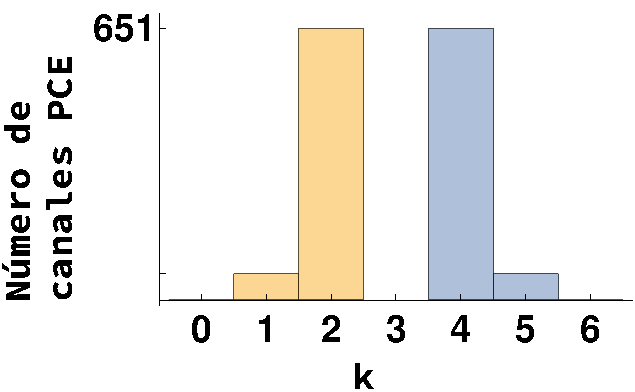
\includegraphics[width=3.7cm]{mirroring_3qubits}
		\hspace*{\fill}
		\caption{3 qubits}
		\label{fig:mirroring_3qubits}
	\end{subfigure}
	\label{fig:mirroring}
\end{figure} % }}}
\end{frame}

\section{Canales de Pauli constantes sobre los ejes}
\begin{frame}{Canales de Ruskai}
	¿Son los canales cuánticos PCE un subconjunto contenido dentro de 
	otro conjunto de canales de Pauli estudiados antes? Especificamente,
	¿son un sobconjunto de los canales de Pauli constantes sobre los ejes\footnote{
	M. Nathanson and M.B. Ruskai, arXiv:quant-ph/0611106 (2006)}? \vfill
	
	No. Cuando mucho existe una intersección no vacía entre ambos 
	canales de Pauli, pero mostramos que ningún conjunto está 
	completamente contenido dentro	del otro.
\end{frame}

\begin{frame}[t]{Conclusiones y trabajo futuro}
	\begin{itemize}
		\item Propusimos estudiar un tipo de canales cuánticos que generalizan  
		las decoherencias de una partícula de dos niveles (qubit) para sistemas de
		$n$ qubits.
		\item Nuestros resultados (regla $2^k$, regla espejo, clases de equivalencia) 
		muestran que los canales cuánticos PCE obedecen alguna estructura matemática.
		\item De hecho, los resultados de este trabajo motivaron a estudiar 
		la diagonalización de la matriz de Choi de las operaciones PCE y 
		a buscar cuál es la estructura matemática de los canales cuánticos PCE.
		\vspace*{1mm}\begin{center}
		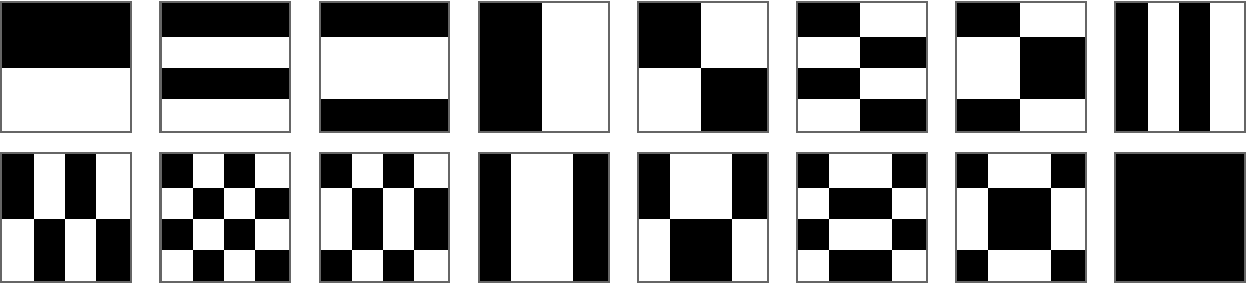
\includegraphics[height=12mm]{portada}
		\end{center}
		\item Actualmente, estamos estudiando una forma de generalizar las 
		operaciones PCE para sistemas de $d$ niveles. 
	\end{itemize}
	
%	\begin{tikzpicture}[x=1mm,y=1mm,overlay,remember picture]
%    \pgftransformshift{\pgfpointanchor{current page}{center}}
%%    \node[inner sep=0pt] (usac) at (-40,-14.5) %
%%    {
\includegraphics[height=14mm]{logos/ecfmByN}};
%%    \node[inner sep=0pt] (usac) at (39,-14.5) %
%%    {
\includegraphics[height=14mm]{logos/ifunam}};
%    \node[inner sep=0pt] (usac) at (0,-30) %
%    {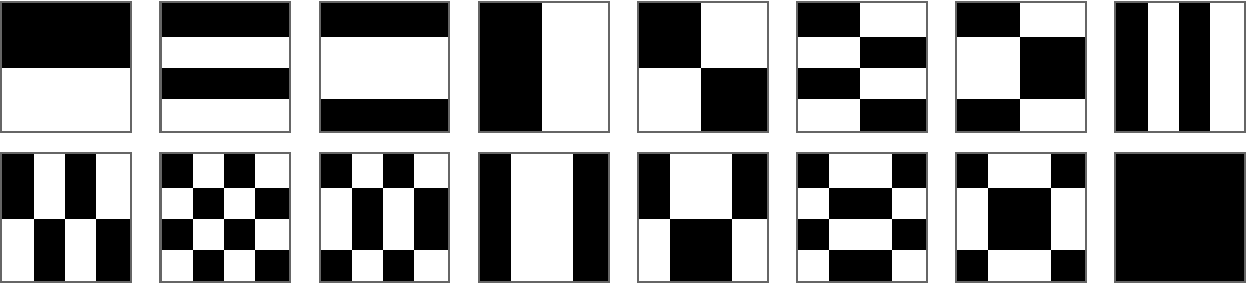
\includegraphics[height=14mm]{portada}};
%    \node[inner sep=0pt] (usac) at (50,-30) %
%    {¡gracias!};
%  \end{tikzpicture}
%	\onslide<2>{
	\hfill \Large \bf ¡Muchas gracias!
%	}
\end{frame}

\end{document}
